\documentclass[sigconf,anonymous]{acmart}

\setcopyright{none}
\settopmatter{printacmref=true}
\renewcommand\footnotetextcopyrightpermission[1]{}
\pagestyle{plain}
\raggedbottom
\setlength{\headheight}{16pt}

\usepackage{booktabs}
\usepackage{graphicx}
\usepackage{xcolor}
\usepackage{microtype}
\usepackage{siunitx}
\usepackage{xspace}

\definecolor{PaperWhite}{HTML}{FFFFFF}
\definecolor{BodyBlack}{HTML}{111827}
\definecolor{RuleBlue}{HTML}{17324D}
\pagecolor{PaperWhite}
\color{BodyBlack}
\hypersetup{colorlinks=true,linkcolor=BodyBlack,citecolor=BodyBlack,urlcolor=RuleBlue}

\newcommand{\bps}[1]{#1~bp}
% Generated by scripts/build_paper_assets.py; do not edit by hand.
% Values are computed only from validated, hashed inputs.
\newcommand{\AdverseEconomicConfirmedCount}{3}
\newcommand{\AdverseHolmPositiveCount}{6}
\newcommand{\AdverseMedianAlphaPct}{10.77\%}
\newcommand{\AdverseNominalPositiveCount}{13}
\newcommand{\AllCountryPositiveCount}{20}
\newcommand{\AlphaIQRPct}{[3.39\%, 9.65\%]}
\newcommand{\AnalysisLockShort}{dba132b6366e}
\newcommand{\ArtifactCountFT}{21}
\newcommand{\ArtifactRateFT}{31.3\%}
\newcommand{\ArtifactTierSummaryFT}{\artifacttier{R0}: 48, \artifacttier{R1}: 6, \artifacttier{R2}: 5, \artifacttier{R3}: 8}
\newcommand{\ArtifactWilsonFT}{[21.51\%, 43.20\%]}
\newcommand{\BHPositiveCount}{18}
\newcommand{\BYPositiveCount}{13}
\newcommand{\BestAdjustedSummary}{Holm $p<0.001$ and max-$|t|$ $p<0.001$}
\newcommand{\BestAlphaPct}{12.25\%}
\newcommand{\BestCandidateLooRangePct}{[9.07\%, 14.49\%]}
\newcommand{\BestCandidateName}{P-F18BC1 014 FactorMAD}
\newcommand{\BestCountry}{FRA}
\newcommand{\BlockSensitivitySummary}{At circular block lengths 3, 6, and 12 months, positive max-$|t|$ discovery counts are 11, 12, 12, while simultaneous 2-percentage-point confirmation counts are 4, 4, 4, respectively.}
\newcommand{\BootstrapCount}{2000}
\newcommand{\BreakEvenBelowTenCount}{1}
\newcommand{\ConclusionResult}{11 Holm and 12 paired max-$|t|$ positive discoveries among 27 executable paths; 35 failed paths remain in the 62-hypothesis Holm/FDR families with $p=1$}
\newcommand{\EconomicConfirmedCount}{4}
\newcommand{\HACSensitivitySummary}{Across fixed HAC lags 0, 3, 6, and 12, nominal-positive counts are 21, 21, 21, 22; Holm counts are 10, 11, 10, 10; BH counts are 17, 18, 18, 19; and BY counts are 13, 13, 13, 13, respectively.}
\newcommand{\HolmPositiveCount}{11}
\newcommand{\JointlyEstimableCount}{27}
\newcommand{\LicensedArtifactCountFT}{10}
\newcommand{\MaxLeaveOneOutMedianShiftPct}{3.07\%}
\newcommand{\MaxMissingExposure}{77.98\%}
\newcommand{\MaxTPositiveCount}{12}
\newcommand{\MedianAlphaPct}{7.62\%}
\newcommand{\MedianCostDragPct}{1.19\%}
\newcommand{\MedianMissingExposure}{0.31\%}
\newcommand{\MedianPositiveCountries}{6}
\newcommand{\MedianTurnover}{0.91}
\newcommand{\MethodSystemCount}{67}
\newcommand{\MissingExposurePninetyfive}{0.69\%}
\newcommand{\NativeDatedOutputCount}{3}
\newcommand{\NativeReturnCount}{0}
\newcommand{\NativeUnavailableCount}{67}
\newcommand{\NoCountryPositiveCount}{0}
\newcommand{\NominalPositiveCount}{21}
\newcommand{\PathFailureCandidateCount}{35}
\newcommand{\PathFailureEventCount}{40}
\newcommand{\PinnedRepoCountFT}{19}
\newcommand{\PositiveAlphaCount}{24}
\newcommand{\PositiveAtFifty}{19}
\newcommand{\PositiveAtTwentyFive}{23}
\newcommand{\ProtocolDeviationStatement}{Two post-lock evaluator amendments are disclosed: Amendment~1 was a post-outcome correctness repair for formation availability, drift, country pooling, and common-calendar defects; Amendment~2 was a subsequent post-runtime complete-path limited-liability rule after a nonpositive-NAV runtime failure. Superseded outputs are archived and excluded.}
\newcommand{\ProxyCount}{62}
\newcommand{\ReachableArtifactCountFT}{19}
\newcommand{\RealityCheckP}{$<0.001$}
\newcommand{\RegressionEndMonth}{December 2024}
\newcommand{\RegressionMonthCount}{293}
\newcommand{\RegressionStartMonth}{August 2000}
\newcommand{\ResultHeadline}{11 Holm and 12 paired max-$|t|$ positive discoveries among 27 executable paths; 35 failed paths remain in the 62-hypothesis Holm/FDR families with $p=1$}
\newcommand{\ResultInterpretation}{11 Holm and 12 paired max-$|t|$ positive discoveries among 27 executable paths; 35 failed paths remain in the 62-hypothesis Holm/FDR families with $p=1$}
\newcommand{\SameWindowGSevenNominalPositiveCount}{22}
\newcommand{\SameWindowSignAgreementCount}{12 of 27}
\newcommand{\SameWindowUSGSevenSpearman}{0.413}
\newcommand{\SignAgreementCount}{13 of 27}
\newcommand{\SystemCount}{103}
\newcommand{\TargetedAuditCount}{25}
\newcommand{\TranslatableSeedCount}{1}
\newcommand{\TurnoverIQR}{0.74--1.33}
\newcommand{\USGSevenSpearman}{0.392}
\newcommand{\USNominalPositiveCount}{6}
\newcommand{\ValidProxyCount}{27}
\newcommand{\WorstAlphaPct}{-7.19\%}
\newcommand{\WorstCandidateName}{P-02FC0B 025 QuantAgent HFT}
\newcommand{\WorstCountry}{JPN}

% Generated by scripts/build_icaif2026_submission_assets.py; do not edit by hand.
% U.S.-primary values are computed from hash-verified frozen outputs.
\newcommand{\USRegressionMonthCount}{281\xspace}
\newcommand{\USRegressionStartMonth}{August 2001\xspace}
\newcommand{\USRegressionEndMonth}{December 2024\xspace}
\newcommand{\USMedianAlphaPct}{-0.05\%\xspace}
\newcommand{\USAlphaIQRPct}{[-1.26\%, 2.05\%]\xspace}
\newcommand{\USPositiveAlphaCount}{30\xspace}
\newcommand{\USNominalCount}{6\xspace}
\newcommand{\USHolmPositiveCount}{1\xspace}
\newcommand{\USMaxTPositiveCount}{1\xspace}
\newcommand{\USEconomicConfirmedCount}{0\xspace}
\newcommand{\USRealityCheckP}{0.0105\xspace}
\newcommand{\USBestAlphaPct}{6.93\%\xspace}
\newcommand{\USBestSimultaneousLowerPct}{0.48\%\xspace}
\newcommand{\USMedianTurnover}{0.90\xspace}
\newcommand{\USTurnoverIQR}{0.63--1.92\xspace}
\newcommand{\USMedianCostDragPct}{1.17\%\xspace}
\newcommand{\USCrossSectionMedianCostShiftPct}{2.20\%\xspace}
\newcommand{\USPositiveAtZero}{46\xspace}
\newcommand{\USPositiveAtFive}{42\xspace}
\newcommand{\USPositiveAtTen}{30\xspace}
\newcommand{\USPositiveAtTwentyFive}{18\xspace}
\newcommand{\USPositiveAtFifty}{10\xspace}
\newcommand{\USMedianGrossAlphaPct}{2.15\%\xspace}
\newcommand{\USHACLagNominalCounts}{5/6/6/6\xspace}
\newcommand{\USHACLagHolmCounts}{0/1/1/0\xspace}
\newcommand{\BroadEvaluationMonthCount}{126\xspace}
\newcommand{\BroadEvaluationStartMonth}{August 2011\xspace}
\newcommand{\BroadEvaluationEndMonth}{January 2022\xspace}
\newcommand{\BroadPositiveAlphaCount}{23\xspace}
\newcommand{\BroadNominalPositiveCount}{1\xspace}
\newcommand{\BroadHolmPositiveCount}{0\xspace}
\newcommand{\BroadMaxTPositiveCount}{0\xspace}
\newcommand{\BroadEconomicConfirmedCount}{0\xspace}
\newcommand{\BroadBestAlphaPct}{9.24\%\xspace}
\newcommand{\BroadBestRawP}{0.0025\xspace}
\newcommand{\BroadBestHolmP}{0.152\xspace}
\newcommand{\BroadBestMaxTP}{0.091\xspace}
\newcommand{\BroadBestSimultaneousLowerPct}{-0.70\%\xspace}
\newcommand{\BroadMarketAlignmentCorrelation}{0.999\xspace}
\newcommand{\MappingNarrativeCount}{49\xspace}
\newcommand{\MappingPartialCount}{12\xspace}
\newcommand{\MappingReleasedSeedCount}{1\xspace}
\newcommand{\MappingAlternativeCandidateCount}{15\xspace}
\newcommand{\MappingCombinationCount}{144\xspace}
\newcommand{\InternationalFailureEventCount}{40\xspace}
\newcommand{\InternationalFailureCandidateCount}{35\xspace}
\newcommand{\InternationalExtremeShortCount}{40\xspace}
\newcommand{\InternationalTwoCellCount}{24\xspace}


\title{Does Public Evidence Support Financial-Agent Alpha Claims?\\An Artifact Audit and Historical Spanning Test}

\author{Anonymous Author(s)}
\affiliation{\institution{Anonymous Institution}}

\acmConference[ICAIF '26]{7th ACM International Conference on AI in Finance}{November 14--17, 2026}{Milan, Italy}
\acmYear{2026}
\copyrightyear{2026}
\acmDOI{}

\begin{abstract}
Financial-agent papers increasingly report profitable factors and trading policies, yet public evidence rarely permits independent alpha testing. We contribute an evidence hierarchy, a system-level artifact census, and a common historical spanning test that keeps reproducibility failures distinct from performance failures. Among 67 formula-discovery or trading systems, 20 list a public artifact and three ship dated native output, but none ships output compatible with our common U.S. equity task. Of 14 targeted implementation attempts, one yields a testable code-backed adaptation; its released seed-expression proxy does not beat a six-factor benchmark. We then audit 62 researcher-authored U.S. mechanism mappings from 51 source indices. These are historical translations, not native agent returns: 49 rely on narrative interpretation, the mappings were frozen after U.S. outcomes had been inspected, and no independent second coder was used. Over August 2001--December 2024, median annualized six-factor alpha net of 10-basis-point one-way costs is \USMedianAlphaPct. Six estimates are nominally positive and one survives familywise correction, but the familywise result is absent at Newey--West lags 0 and 12; no simultaneous lower bound exceeds a two-percentage-point reporting threshold. A post-hoc 133-factor rolling spanning diagnostic yields no familywise discovery. Finally, security-level reconstruction shows that all \InternationalFailureEventCount international insolvency events are dominated by a single extreme positive return on a short position, so we exclude international performance from the headline evidence. Public artifacts and favorable historical mappings therefore do not establish broad, economically material U.S. alpha. The contribution is an auditable method for separating unavailable evidence, lower-fidelity economic tests, and benchmark failure.
\end{abstract}

\ccsdesc[500]{Computing methodologies~Multi-agent systems}
\ccsdesc[500]{Applied computing~Economics}
\ccsdesc[300]{General and reference~Empirical studies}

\keywords{financial agents, alpha, asset pricing, reproducibility, multiple testing, empirical audit}

\begin{document}
\maketitle

\section{Introduction}

Financial AI systems now search factor expressions, debate investment theses, retrieve news, and revise portfolios. Their evaluations often report Sharpe ratios, raw trading gains, benchmark outperformance, or alpha \cite{LiEtAl2024FAMA,TangEtAl2025AlphaAgent,WangEtAl2025AlphaGPT,ZhangEtAl2026QuantEvolver,DuanEtAl2025FactorMAD}. The scientific question is not whether these architectures are interesting. It is whether the evidence released with them supports the claimed incremental return.

That question contains two different failure modes. A system may be impossible to evaluate because its code, data adapter, trained state, or dated output is unavailable. Alternatively, a testable return path may exist but fail an asset-pricing benchmark. Treating both as zero alpha is wrong; stopping at ``not reproducible'' is also incomplete. We therefore use the highest-fidelity feasible route and label the estimand at every step. Native or code-backed returns, when available, test a released implementation. When they are unavailable, a transparent mechanism mapping can test whether the documented economic idea spans familiar factors. It cannot identify an agent's contribution.

This distinction changes the paper's claim. We do not test whether financial agents, as a class, can discover alpha. We test whether their \emph{public evidence} establishes alpha under an independently specified common task. Our U.S. portfolio results are retrospective historical spanning diagnostics conditional on researcher-authored mappings. They do not demonstrate prospective discovery and cannot correct for prior factor mining or publication selection \cite{HarveyLiuZhu2016,BaileyEtAl2017PBO}.

We make four contributions. First, a 67-system artifact census records public availability, pinned revisions, native dated output, and exact blocking stages. Second, a direct-code audit separates one testable adaptation from 13 non-evaluable attempts. Third, a row-level mapping ledger exposes every formula, source-support category, omitted component, freeze hash, and alternative already coded. Fourth, we subject 62 U.S. mappings to trading costs, six-factor and broad-factor spanning, familywise inference, and explicit sensitivity tests. The central empirical finding is not ``no strategy works.'' It is narrower and more useful: the released evidence does not establish broad, economically material U.S. alpha, and the one primary familywise result is specification-fragile.

\begin{figure*}[t]
  \centering
  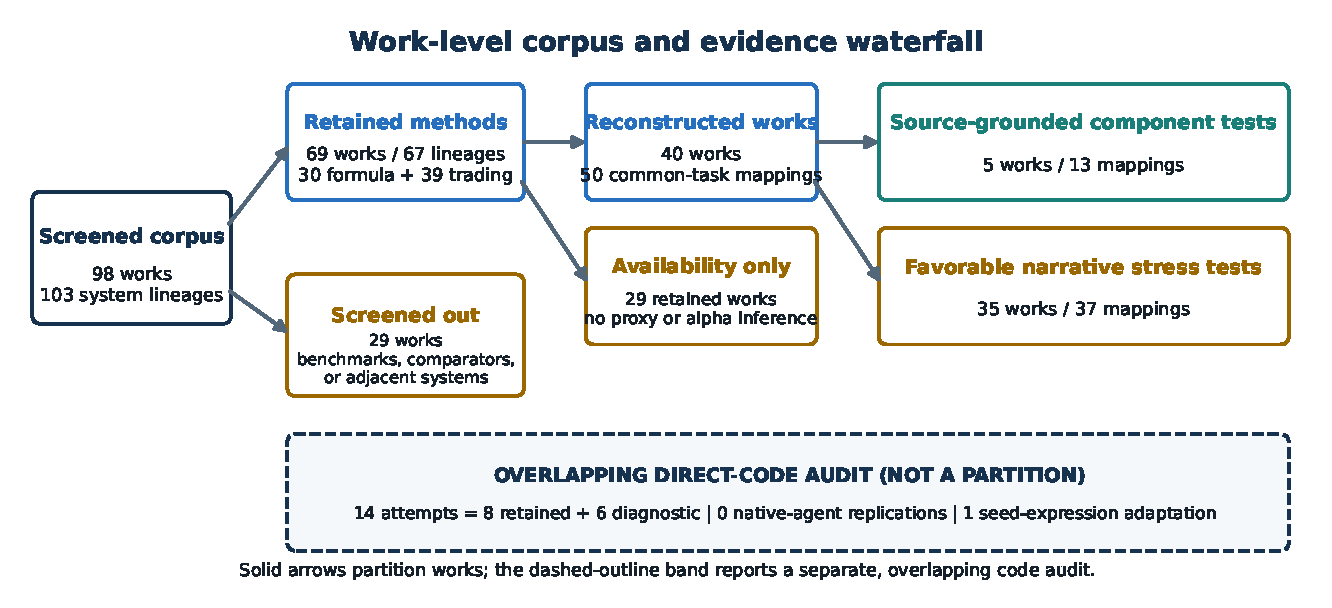
\includegraphics[width=0.92\textwidth]{figures/claim_to_test_pipeline.pdf}
  \caption{Evidence routes and estimands. A missing native path is an evidence failure, not a zero return. A mechanism mapping tests historical economic content, not agent performance. FWE denotes familywise-error-controlled inference.}
  \Description{Two routes from public financial-agent claims. Fourteen implementation attempts yield one testable adaptation and no six-factor beater. Fifty-one source indices yield 62 researcher-authored U.S. mappings, one conditional six-factor familywise result, and no broad-factor familywise result.}
  \label{fig:pipeline}
\end{figure*}

\section{Evidence Design}

\subsection{Denominators and inferential targets}

The three headline denominators are related but not interchangeable. The census contains 67 formula-discovery or trading systems. A separate source-discovery corpus contains 55 indexed records suitable for economic coding; 51 indices are translated into 62 candidate portfolios because five sources have multiple already-coded interpretations. One index names two systems, so the ledger has 52 named source rows. The 62 portfolios are the statistical family. None of the 51 mapped sources contains an explicit exact match to the full common claim ``monthly U.S. top-1,000 equity alpha relative to our six-factor model.'' Consequently, our outcome is a common-task spanning result, not a reproduction of 51 identically stated original alpha claims.

The 14 targeted repositories are a diagnostic subset of public implementations, not the nine artifacts with an observed reuse license. License presence is a census field; the execution audit also inspected locally available public snapshots without redistributing them. We report 0 of 1 testable code-backed paths beating the benchmark. The remaining 13 attempts are classified by blocking stage and never enter a performance denominator.

\begin{table}[t]
\centering
\caption{Evidence hierarchy and what each result identifies.}
\label{tab:hierarchy}
\small
\begin{tabular}{p{0.20\columnwidth}p{0.29\columnwidth}p{0.39\columnwidth}}
\toprule
\textbf{Stage} & \textbf{Evidence/result} & \textbf{Permitted interpretation} \\
\midrule
System census & 67 systems; 20 artifacts; 3 dated outputs & Public evidence availability only \\
Targeted code audit & 14 attempts; 1 testable, 13 non-evaluable & 0 of 1 beats six factors; no performance claim for 13 \\
Mechanism mapping & 62 mappings; 1 primary FWE, 0 material & Conditional historical spanning of researcher mappings \\
Broad diagnostic & 133 factors; 0 FWE results & Post-hoc diagnostic, not confirmatory evidence \\
International forensic audit & 40 events; all dominated by one short-held return & Data/implementation alarm; no performance inference \\
\bottomrule
\end{tabular}
\end{table}

\subsection{Artifact and direct-code route}

We freeze repository URLs and revisions, record whether dated signals, positions, or returns are shipped, and classify a public path as native only when it represents the released system rather than an analyst-authored substitute. Of 67 systems, 20 list an artifact, 18 are reachable at the audit date, nine have an observed reuse license, and three contain dated native output. Those three outputs concern different assets or tasks; none is compatible with the common panel.

We attempted 14 implementations selected for apparent code availability and relevance. Twelve contain public code, one is ambiguous unofficial code, and one is a placeholder. The sole computable adaptation is a QuantEvolver released seed expression evaluated on the JKP panel, not a trained QuantEvolver agent. Its annualized six-factor alpha is 0.33\% ($t=0.65$), so it does not beat the benchmark. The package preserves the 13 blocking records separately: absent native output, missing inputs or adapters, incompatible task, or non-executable artifact. This makes the negative performance denominator one, not fourteen.

\subsection{Mechanism mapping and disclosed discretion}

When direct evaluation is unavailable, we map public descriptions to point-in-time JKP characteristics \cite{JensenKellyPedersen2023}. Each row in the supplement records the source index and category, source name, economic rationale, exact score, portfolio rule, source support for ingredients/signs/weighting, original domain mismatch, omitted agent components, and evidence category. The coding tiers are shown in Table~\ref{tab:mapping}. A narrative translation is deliberately labeled M0 even when economically favorable.

\begin{table}[t]
\centering
\caption{Mapping fidelity and U.S. results by tier.}
\label{tab:mapping}
\small
\begin{tabular}{lrrr}
\toprule
\textbf{Evidence tier} & \textbf{$N$} & \textbf{Median alpha} & \textbf{Holm $+$} \\
\midrule
M0 narrative translation & 49 & $-0.10\%$ & 1 \\
M1 example/motif support & 6 & $-0.71\%$ & 0 \\
M1 named-rule support & 6 & $3.12\%$ & 0 \\
M2 released seed expression & 1 & $-0.28\%$ & 0 \\
\bottomrule
\end{tabular}
\par\vspace{0.2em}\footnotesize Annualized six-factor alpha net of \bps{10} one-way costs. ``Holm $+$'' counts positive estimates surviving Holm at 5\%.
\end{table}

The ledger makes three adverse facts explicit. First, \MappingNarrativeCount mappings are narrative translations and \MappingPartialCount have partial source support; only one uses a released expression. Second, the registry hash was frozen on 3 August 2026 after U.S. outcomes had already been inspected. The coding is therefore not outcome-blind, notwithstanding its immutable final hash. Third, no independent second coder was used. The reported p-values quantify sampling variation conditional on these formulas; they do not incorporate mapping discretion.

We can measure only a lower bound on that discretion. Five sources already have multiple coded mappings, covering \MappingAlternativeCandidateCount candidates. Selecting one mapping per source yields \MappingCombinationCount combinations; the same AlphaAgent-inspired quality proxy is the sole Holm discovery in every combination. This does not validate singly mapped formulas, nor does it replace independent coding. It shows only that the headline count is unchanged within the alternatives that happened to be coded.

\subsection{Common U.S. task and estimators}

The primary panel is monthly U.S. common equity from August 2001 through December 2024. At each formation month we retain the 1,000 largest positive-market-equity securities, compute signals using information available at formation, and hold for the next month. Most mappings are value-weighted top-minus-bottom deciles; long-only mappings are explicitly labeled. Long and short legs each carry unit notional, so a long-short portfolio has gross exposure two. Missing realized returns are zero-filled under the locked primary policy and audited separately.

Turnover uses drifted pre-trade weights. Candidate returns are net of \bps{10} per unit of traded notional one way. We do not model borrow fees, financing, locate constraints, nonlinear impact, or capacity. Excess returns use the risk-free rate for the cash component. The market, size, value, investment, profitability, and momentum benchmark factors are gross, not charged the candidate cost model. Thus the test asks whether an implementable-cost candidate beats standard published gross factors; it is not a symmetric comparison of two equally costed tradable products.

For candidate $i$ we estimate
\[
r_{i,t}^{\mathrm{net}}=\alpha_i+\beta_i' f_t+\varepsilon_{i,t}.
\]
The primary Newey--West lag is the automatic rule $\lfloor4(T/100)^{2/9}\rfloor$ (four at $T=281$) \cite{NeweyWest1987}. We report two-sided nominal tests, Holm correction across all 62 candidates \cite{Holm1979}, and paired moving-block maximum-$|t|$ inference with 2,000 bootstrap replications and a six-month block. Block lengths three and twelve and HAC lags 0, 3, 6, and 12 are sensitivities. A simultaneous lower bound of at least two annual percentage points is a pragmatic reporting threshold selected by the project owner after U.S. outcomes were available; it is not a preregistered decision rule.

\section{Results}

\subsection{Primary U.S. historical spanning test}

All 62 paths are executable for \USRegressionMonthCount months. At \bps{10}, median annualized six-factor alpha is \USMedianAlphaPct (interquartile range \USAlphaIQRPct); \USPositiveAlphaCount point estimates are positive, \USNominalCount are nominally significant, and \USHolmPositiveCount survives Holm and paired maximum-$|t|$ inference. No simultaneous lower bound exceeds two percentage points. The largest estimate, 6.93\%, belongs to a \emph{researcher-authored AlphaAgent-inspired quality mechanism proxy}; the software did not generate this portfolio, and its simultaneous lower bound is only 0.48\%.

The apparent discovery is fragile to serial-correlation choices. Across fixed Newey--West lags 0/3/6/12, nominal positive counts are \USHACLagNominalCounts and Holm counts are \USHACLagHolmCounts. The familywise result therefore exists at lags 3 and 6 but not at 0 or 12. Block-length changes leave the maximum-statistic count at one, but that does not cure mapping or publication-selection uncertainty.

Trading costs explain much of the cross-section. Median gross alpha is \USMedianGrossAlphaPct, compared with \USMedianAlphaPct at \bps{10}; median candidate-level cost drag is \USMedianCostDragPct. Positive-alpha counts fall from \USPositiveAtZero at zero cost to \USPositiveAtFive, \USPositiveAtTen, \USPositiveAtTwentyFive, and \USPositiveAtFifty at 5, 10, 25, and 50 basis points (Figure~\ref{fig:cost}).

\begin{figure}[t]
  \centering
  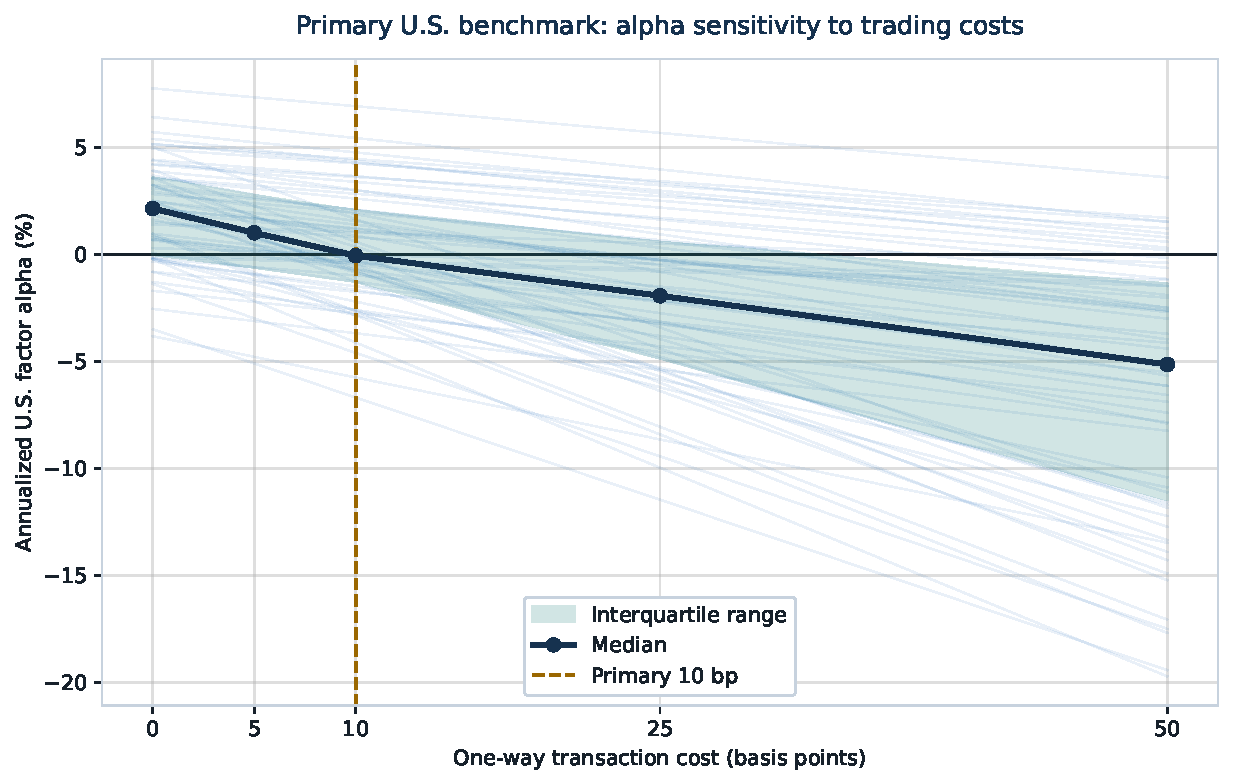
\includegraphics[width=\columnwidth]{figures/usa_cost_sensitivity.pdf}
  \caption{Annualized six-factor alpha across one-way trading-cost assumptions. Thin lines are candidate mappings; the band is the interquartile range. Benchmark factors remain gross.}
  \Description{Candidate alphas generally decline as one-way trading costs rise from zero to fifty basis points. The median crosses slightly below zero at ten basis points.}
  \label{fig:cost}
\end{figure}

These results support a precise finding: favorable characteristic translations rarely provide economically material incremental U.S. return after costs and search-wide inference. They do not show that the unavailable native agents would earn the same returns, and they do not establish prospective discovery.

\subsection{Post-hoc broad-factor diagnostic}

The broader diagnostic uses the market plus 132 JKP characteristic factors. Its source factor panel ends in December 2021; factors are shifted to the candidate return month, yielding a common panel through January 2022. With a 120-month trailing window, evaluation therefore runs from August 2011 through January 2022 (\BroadEvaluationMonthCount months), not through 2024. The shorter sample is a data-availability constraint, not an unexplained loss of candidate observations.

At each evaluation month, the ridge penalty is selected anew from past data: 96 months for fitting and 24 for validation, with the low-dimensional core unpenalized. The selected model is refit on all 120 past months and produces a one-month-ahead residual. The 5,000-replication moving-block bootstrap resamples centered, already-estimated out-of-sample residuals; it does \emph{not} rerun rolling estimation or penalty selection. Its uncertainty is conditional on the realized fitting path and may be optimistic. This analysis was designed after primary outcomes and is descriptive, not a robustness confirmation.

There are \BroadPositiveAlphaCount positive estimates and one nominal result, but zero Holm discoveries, zero maximum-$|t|$ discoveries, and zero simultaneous lower bounds above two percentage points. The best raw $p$-value is \BroadBestRawP; its Holm value is \BroadBestHolmP and maximum-statistic value is \BroadBestMaxTP. This strengthens the spanning interpretation, but only as post-hoc evidence over the truncated period.

\subsection{International extension: forensic result, not alpha evidence}

The international extension is excluded from headline performance inference. Thirty-five of 62 paths cross nonpositive net asset value, producing \InternationalFailureEventCount events: 31 in France, five in Canada, two in Germany, one in Britain, and one in Italy. Security-level reconstruction reproduces every recorded event to numerical tolerance. In all \InternationalExtremeShortCount cases, one extreme positive security return held on the short side accounts for at least half of the portfolio loss. Two France return-month cells contain \InternationalTwoCellCount events; the largest held returns reach implausibly extreme multiples.

As a diagnostic, capping individual security total returns at +100\% eliminates all insolvency events; caps of +200\%, +500\%, and +1,000\% leave 1, 1, and 7 events. These caps are not an admissible corrected return policy and are not used to report alpha. The concentration could reflect corporate actions, return construction, stale prices, or interactions between short weights and extreme observations. Without independent security-level validation, the extension is a data/implementation alarm. The supplement preserves every event, security identifier, weight, return, contribution, reconstruction error, and cap diagnostic.

\section{What the Evidence Does and Does Not Establish}

The results have scientific value in three places. First, they quantify the gap between a paper claim and an inspectable return stream. Only one of 14 targeted implementations reaches a common code-backed performance test, while the other 13 remain auditable evidence failures. Second, they show that recognizable economic stories can be tested even when native execution is impossible, provided those tests are labeled as lower fidelity. Third, they demonstrate how costs, factor breadth, and familywise inference change conclusions that would look positive under gross returns and nominal tests.

The design also has firm limits. Many systems were released after the December 2024 end of the U.S. return panel. We do not claim a publication-date out-of-sample test: there are too few or zero post-release months for much of the corpus, and the mappings themselves were frozen in 2026 after outcome inspection. The historical tests cannot distinguish discovery from repackaging of known characteristics. Holm correction controls sampling multiplicity across the 62 fixed mappings; it does not correct the literature's search process, the unpublished mapping universe, or publication selection.

Common-task comparability also trades away native fidelity. Monthly top-1,000 characteristic portfolios omit language generation, memory, retrieval, debate, timing, daily or intraday execution, dynamic risk allocation, non-equity instruments, and tool-driven adaptation. A mapping failure cannot prove that its native agent fails; a mapping success cannot be attributed to an agent. Table~\ref{tab:mapping} shows that the strongest-looking M0 result is precisely in the lowest-fidelity class.

These limits motivate a release standard for future financial-agent work: revision-pinned code; an environment manifest; immutable dated signals, positions, or returns; universe and timing rules; cost and financing conventions; model, prompt, and seed versions; search breadth and failed-candidate counts; and original benchmark definitions. An agentic contribution further requires provenance or ablation that separates the agent from its factor library and human-authored search space.

\section{Anonymous Empirical Artifact}

The submission package is designed to make the audit inspectable without redistributing restricted security-level data. It contains the 67-system census, the 55-source ledger, all 62 formulas, source-support and fidelity fields, the freeze timestamp and hash, repository screening decisions, execution-status logs, aggregate monthly U.S. candidate and factor returns, turnover and cost outputs, broad-factor residuals, multiplicity results, international event forensics, superseded-run notices, analysis scripts, tests, manifests, and a machine-readable inventory of SHA-256 hashes. The row-level mapping ledger states explicitly that mappings were not outcome-blind and had no second coder. Restricted raw market data are referenced by source path and input hash rather than redistributed.

Deterministic builders regenerate manuscript macros and figures from hash-verified outputs. Tests cover timing, portfolio weights, drift, costs, HAC calculations, familywise adjustments, mapping-combination sensitivity, and international event reconstruction. This artifact is part of the contribution: hashes establish integrity only because the underlying aggregate objects and code are included.

\paragraph{Responsible use and AI assistance.}
No orders were transmitted. Results are retrospective research evidence, not investment advice. Generative AI assisted literature organization, code drafting, diagnostic review, and prose editing; the human author is responsible for source selection, mappings, protocol choices, statistical specifications, citation verification, and all reported claims.

\section{Conclusion}

Public financial-agent evidence does not currently establish broad, economically material U.S. alpha. The direct-code route yields one testable adaptation and no benchmark beater; 13 other attempts are reproducibility or compatibility failures, not negative returns. The lower-fidelity route yields 62 transparent historical mappings, one specification-fragile six-factor familywise result, no effect clearing the materiality threshold, and no familywise result in a post-hoc broad-factor diagnostic. The international extension fails a security-level plausibility audit and is not used as performance evidence.

The paper's contribution is therefore constructive rather than categorical. It supplies an evidence hierarchy and an inspectable workflow for determining what public artifacts can support, for pursuing the economic content of otherwise non-evaluable claims, and for stopping the interpretation exactly where fidelity and design no longer permit it.

\bibliographystyle{ACM-Reference-Format}
\bibliography{icaif2026_references}

\end{document}
